\documentclass[10pt,aspectratio=149]{beamer}

% All the boilerplate is in ac1slides.sty
% Note that this also pulls in a custom vogtwidebar.sty
\usepackage{ac1slides}

\author{Ji\v{r}\'i Lebl}

\institute[OSU]{%
Departemento pri Matematiko de Oklahoma {\^S}tata Universitato}

\title{BA: 7.5}

\date{}

\begin{document}

\begin{frame}
\titlepage
\end{frame}

\begin{frame}
\begin{definition}
Let $(X,d_X)$ and $(Y,d_Y)$ be metric spaces and $c \in X$.

\pause
$f \colon X \to Y$ is
\emph{continuous at $c$} if

\pause
$\forall$ $\epsilon > 0$
$\exists$ $\delta > 0$ s.t. whenever $x \in X$ and $d_X(x,c) < \delta$, then
$d_Y\bigl(f(x),f(c)\bigr) < \epsilon$.

\pause
\medskip

If $f \colon X \to Y$ is continuous at all $c \in X$, then
$f$ is a \emph{continuous function}.
\end{definition}

\pause
\begin{proposition}
Let $(X,d_X)$ and $(Y,d_Y)$ be metric spaces.
\pause
Then $f \colon X \to Y$ is
continuous at $c \in X$
\pause
\wiffif for every $\{ x_n \}_{n=1}^\infty$ in $X$
converging to $c$, $\bigl\{ f(x_n) \bigr\}_{n=1}^\infty$ converges
to $f(c)$.
\end{proposition}

\pause
\textbf{Proof:}
Suppose $f$ is continuous at $c$ and $\{ x_n \}_{n=1}^\infty$ converges to
$c$.

\pause
Given $\epsilon > 0$, $\exists$ $\delta > 0$ s.t. $d_X(x,c) < \delta$ implies
$d_Y\bigl(f(x),f(c)\bigr) < \epsilon$.

\pause
Take $M$ such that 
$\forall$ $n \geq M$, ~$d_X(x_n,c) < \delta$

\pause
\thus \quad $\forall$ $n \geq M$, ~$d_Y\bigl(f(x_n),f(c)\bigr) < \epsilon$
\pause
\wthus $\bigl\{ f(x_n) \bigr\}_{n=1}^\infty$
converges to $f(c)$.

\pause
\medskip

Now suppose $f$ is not continuous at $c$.

\pause
$\exists$ $\epsilon > 0$, s.t. for every $n \in \N$ $\exists$ $x_n \in X$,
~$d_X(x_n,c) < \nicefrac{1}{n}$ and $d_Y\bigl(f(x_n),f(c)\bigr) \geq \epsilon$.

\pause
\thus \quad $\{ x_n \}_{n=1}^\infty$ converges to $c$, but
$\bigl\{ f(x_n) \bigr\}_{n=1}^\infty$
does not converge to $f(c)$.
\qed

\end{frame}

\begin{frame}

\textbf{Example:}
Suppose $f \colon \R^2 \to \R$ is a polynomial:
\begin{equation*}
f(x,y) =
\sum_{j=0}^d
\sum_{k=0}^{d-j}
a_{jk}\,x^jy^k =
a_{0\,0} + a_{1\,0} \, x +
a_{0\,1} \, y+  
a_{2\,0} \, x^2+  
a_{1\,1} \, xy+  
a_{0\,2} \, y^2+ \cdots +
a_{0\,d} \, y^d ,
\end{equation*}

\pause
Claim: $f$ is continuous.

\pause
\medskip

Let $\bigl\{ (x_n,y_n) \bigr\}_{n=1}^\infty$ be a sequence in $\R^2$
converging to $(x,y) \in \R^2$.

\pause
\thus \quad
$\lim\limits_{n\to\infty} x_n = x$ and $\lim\limits_{n\to\infty} y_n = y$.

\pause
\medskip

Then
\[
\lim_{n\to\infty}
f(x_n,y_n)
\pause
=
\lim_{n\to\infty}
\sum_{j=0}^d
\sum_{k=0}^{d-j}
a_{jk} \, x_n^jy_n^k 
\pause
=
\sum_{j=0}^d
\sum_{k=0}^{d-j}
a_{jk} \, x^jy^k
\pause
=
f(x,y) .
\]

\pause
\thus \quad $f$ is continuous at $(x,y)$
\pause
\wthus $f$ is continuous.

\end{frame}

\begin{frame}

Careful about taking limits separately in $\R^n$.

\pause

Consider $f(x,y) \coloneqq \frac{xy}{x^2+y^2}$ for $(x,y) \not= (0,0)$ and
$f(0,0) \coloneqq 0$.

\pause
\begin{center}
\scalebox{0.8}{
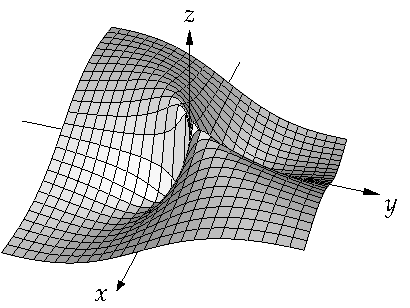
\includegraphics{../figures/xyxsqysq}
}
\end{center}

\pause
\textbf{Exercise:} Prove that $f$ is not continuous at $(0,0)$,

\pause
but that for every fixed $y$, ~~ the function $g(x) \coloneqq f(x,y)$ is
continuous,

\pause
and for every fixed $x$, ~~ $h(y) \coloneqq f(x,y)$ is continuous.


\end{frame}

\begin{frame}

Let $X$ be a metric space and $f \colon X \to \C$ a complex-valued function.

\pause
\medskip

Write $f(p) = g(p) + i \, h(p)$, where $g \colon X \to \R$ and $h \colon X \to \R$.


\pause
\medskip

\textbf{Claim:}
$f$ is continuous at $c \in X$ \wiffif $g$ and $h$ are continuous at $c$.

\pause
\medskip

Claim follows as $\bigl\{ f(p_n) = g(p_n) + i \,h(p_n) \bigr\}_{n=1}^\infty$
converges to $f(p) = g(p) + i \, h(p)$

\pause
\iffif \quad
$\bigl\{ g(p_n) \bigr\}_{n=1}^\infty$ converges to $g(p)$
\pause
and
$\bigl\{ h(p_n) \bigr\}_{n=1}^\infty$ converges to $h(p)$.

\end{frame}

\begin{frame}

Continuous maps do not map closed sets to closed sets.

\pause
E.g., if $f \colon (0,1) \to \R$, ~ $f(x) \coloneqq x$, ~ then
$f\bigl((0,1)\bigr) = (0,1)$,

\pause
but $(0,1)$ is closed in $(0,1)$, but not closed in $\R$.

\pause

\begin{lemma}
Let $(X,d_X)$ and $(Y,d_Y)$ be metric spaces
and $f \colon X \to Y$ a continuous function.

\pause
If $K \subset X$ is compact, then $f(K)$ is compact.
\end{lemma}

\pause
\textbf{Proof:}
A sequence in $f(K)$ can be written as
$\bigl\{ f(x_n) \bigr\}_{n=1}^\infty$, where
$\{ x_n \}_{n=1}^\infty$ is a sequence in $K$.

\pause
\medskip

$K$ is compact \wthus $\exists$
subsequence
$\{ x_{n_j} \}_{j=1}^\infty$ converging to some $x \in K$.

\pause
\medskip

By continuity
$\displaystyle
\lim_{j\to\infty} f(x_{n_j})
\pause
= f(x)
\pause
\in f(K)$.

\pause
\medskip

\thus \quad every sequence in $f(K)$ has a subsequence convergent to 
a point in $f(K)$

\pause
\thus \quad $f(K)$ is (sequentially) compact.
\qed

\end{frame}

\begin{frame}

$f \colon X \to \R$ achieves an
\emph{absolute minimum} at $c \in X$ if
\begin{equation*}
f(x) \geq f(c) \qquad \text{for all } x \in X.
\end{equation*}
\pause
$f$ achieves an 
\emph{absolute maximum} at $c \in X$ if
\begin{equation*}
f(x) \leq f(c) \qquad \text{for all } x \in X.
\end{equation*}

\pause
\begin{theorem}
Let $(X,d)$ be a nonempty compact metric space
and let $f \colon X \to \R$ be continuous.

\pause
\thus ~~
$f$ is bounded and
achieves an absolute minimum and an absolute maximum on~$X$.
\end{theorem}

\pause
\textbf{Proof:}
$X$ is compact and $f$ continuous
\pause
\wthus
$f(X) \subset \R$ is compact.

\pause
Thus $f(X)$ is closed and bounded.

\pause
\thus \quad $\sup f(X) \in f(X)$ ~~and~~ $\inf f(X) \in f(X)$

(both achieved by sequences in $f(X)$, which is closed).

\pause
\medskip

\thus
\quad $\exists$ $x \in X$ s.t. $f(x) = \sup f(X)$
\pause
\quad and \quad
$\exists$ $y \in X$ s.t. $f(y) = \inf f(X)$.
\qed

\end{frame}

\begin{frame}
\begin{lemma}
Let $(X,d_X)$ and $(Y,d_Y)$ be metric spaces.
\pause
$f \colon X \to Y$ is continuous at $c \in X$
\wiffif for every open neighborhood $U$ of $f(c)$ in $Y$,  ~
$f^{-1}(U)$ contains an open neighborhood of $c$ in $X$.
\end{lemma}

\pause
\hfill\scalebox{0.8}{
\subimport*{../figures/}{mscontfuncpt.pdf_t}
}

\vspace*{-1.05in}

\pause
\textbf{Proof:}
Suppose $f$ is continuous at $c$, and

\pause
$U \subset Y$ is an open neighborhood of $f(c)$.

\pause
\thus \quad
$B_Y\bigl(f(c),\epsilon\bigr) \subset U$ for some $\epsilon > 0$.

\pause
$\exists$ $\delta > 0$, s.t. if $d_X(x,c) < \delta$,

\pause
then
$d_Y\bigl(f(x),f(c)\bigr) < \epsilon$.

\pause
I.e.,
$
B_X(c,\delta)
\pause
\subset f^{-1}\bigl(B_Y\bigl(f(c),\epsilon\bigr)\bigr)
\pause
\subset
f^{-1}(U)$,

\pause
and $B_X(c,\delta)$ is an open neighborhood of $c$.

\pause
\medskip

Now let $\epsilon > 0$ be given.

\pause
If $f^{-1}\bigl(B_Y\bigl(f(c),\epsilon\bigr)\bigr)$ contains an open
neighborhood $W$ of $c$, then

\pause
$\exists$ $\delta > 0$, s.t.
$B_X(c,\delta) \subset W \subset
f^{-1}\bigl(B_Y\bigl(f(c),\epsilon\bigr)\bigr)$.

\pause
That means if $d_X(x,c) < \delta$,
then $d_Y\bigl(f(x),f(c)\bigr) < \epsilon$,

\pause
\thus \quad $f$ is continuous at~$c$.
\qed

\end{frame}

\begin{frame}

\begin{theorem}
Let $(X,d_X)$ and $(Y,d_Y)$ be metric spaces.

\pause
$f \colon X \to Y$
is continuous
\wiffif
for every open $U \subset Y$, ~ $f^{-1}(U)$ is open in $X$.
\end{theorem}

\pause
\textbf{Proof:} Exercise.

\end{frame}

\begin{frame}

\textbf{Example:}
If $f \colon X \to Y$ is continuous and $E$ is closed,

\pause
then $f^{-1}(E) = X \setminus f^{-1}(E^c)$ is also closed.

\pause
\medskip

Suppose 
$f \colon X \to \R$ is continuous.

\pause
\medskip

\thus \quad
the 
\emph{zero set} of $f$, ~
$f^{-1}(0) = \bigl\{ x \in X : f(x) = 0 \bigr\}$, ~
is closed.

\pause
\medskip

For example, the zero set of a polynomial is closed.

\pause
\medskip

Similarly, 

\medskip

$f^{-1}\bigl( [0,\infty) \bigr) = \bigl\{ x \in X : f(x) \geq 0 \bigr\}$,
is closed.

\pause
\medskip

$f^{-1}\bigl( (0,\infty) \bigr) = \bigl\{ x \in X : f(x) > 0 \bigr\}$,
is open.  

\end{frame}

\begin{frame}

\begin{definition}
Let $(X,d_X)$ and $(Y,d_Y)$ be metric spaces.
$f \colon X \to Y$ is
\emph{uniformly continuous} if

\pause
$\forall$ $\epsilon > 0$
$\exists$ $\delta > 0$ s.t. whenever $p,q \in X$ and
$d_X(p,q) < \delta$, then
$d_Y\bigl(f(p),f(q)\bigr) < \epsilon$.
\end{definition}

\pause
\begin{theorem}
Let $(X,d_X)$ and $(Y,d_Y)$ be metric spaces.
Suppose $f \colon X \to Y$ is continuous and $X$ is compact.
\pause
Then $f$ is uniformly continuous.
\end{theorem}

\pause
\textbf{Proof:}
Let $\epsilon > 0$ be given.

\pause
$\forall$ $c \in X$,
pick $\delta_c > 0$ s.t.
$d_Y\bigl(f(x),f(c)\bigr) < \nicefrac{\epsilon}{2}$
whenever
$x \in B(c,\delta_c)$.

\pause
$X \subset \bigcup_{c \in X} B(c,\delta_c)$ and $X$ is compact.  

\pause
By Lebesgue covering lemma,

$\exists$ $\delta > 0$
s.t. $\forall$ $x \in X$,
$\exists$ $c \in X$
for which $B(x,\delta) \subset B(c,\delta_c)$.

\pause
\medskip

Suppose $p, q \in X$ where $d_X(p,q) < \delta$.
Find $c \in X$ s.t. $B(p,\delta) \subset B(c,\delta_c)$.

\pause
Then $q \in B(c,\delta_c)$.

\pause
By the triangle inequality
and the definition of $\delta_c$,

\medskip

$
d_Y\bigl(f(p),f(q)\bigr)
\pause
\leq
d_Y\bigl(f(p),f(c)\bigr)
+
d_Y\bigl(f(c),f(q)\bigr)
\pause
<
\nicefrac{\epsilon}{2}+
\nicefrac{\epsilon}{2} = \epsilon$.
\qed

\end{frame}

\begin{frame}

\begin{proposition}
If $f \colon [a,b] \times [c,d] \to \R$ is continuous,
then $g \colon [c,d] \to \R$ defined by
\begin{equation*}
g(y) \coloneqq \int_a^b f(x,y) \,dx  \qquad \text{is continuous}.
\end{equation*}
\end{proposition}

\pause
\textbf{Proof:}
Suppose $y \in [c,d]$.

\pause
\medskip

Let $\epsilon > 0$ be given.

\pause
\medskip

As $[a,b] \times [c,d]$ is compact, $f$
is uniformly continuous.
\pause
~~ So

$\exists$ $\delta > 0$ s.t.
if $z \in [c,d]$ and
$\abs{z-y} < \delta$, then
$\abs{f(x,z)-f(x,y)} < \frac{\epsilon}{b-a}$ ~$\forall$ $x \in [a,b]$.

\pause
\medskip

Suppose $\abs{z-y} < \delta$.
\pause
Then

\medskip

$\displaystyle
\abs{
g(z)-
g(y)
}
\pause
=
\bbabs{
\int_a^b 
f(x,z) \,dx 
-
\int_a^b 
f(x,y) \,dx 
}$

\pause
\medskip

\hfill
\hfill
\hfill
$\displaystyle
=
\bbabs{
\int_a^b 
\bigl(
f(x,z) - f(x,y)
\bigr)
\,dx 
}
\pause
\leq
(b-a)
\frac{\epsilon}{b-a}
\pause
= \epsilon$.
\qed

\end{frame}

\begin{frame}

\textbf{Example:}
Suppose $(X,d_X)$ and $(Y,d_Y)$ are metric spaces.

\pause
\medskip


$f \colon X \to Y$ is \emph{Lipschitz} or \emph{$K$-Lipschitz} if $\exists$
$K \in \R$ s.t.
\[
d_Y\bigl(f(p),f(q)\bigr) \leq K\, d_X(p,q)
\qquad \text{for all } p,q \in X.
\]

\pause
A Lipschitz $f$ is uniformly continuous:
\pause
Take $\delta = \nicefrac{\epsilon}{K}$.

\pause
\medskip

$f$ can be uniformly continuous but not Lipschitz:
\pause
$\sqrt{x}$ on $[0,1]$

\end{frame}

\begin{frame}

\begin{definition}
Let $(X,d)$ be a metric space and
$S \subset X$.

\pause
$p \in X$ is 
a \emph{cluster point} of $S$
if $\forall$ $\epsilon > 0$, ~~$B(p,\epsilon) \cap S
\setminus \{ p \} \not= \emptyset$.
\end{definition}

\pause
\textbf{Exercise:}
$p \in X$ is a cluster point of $S$  \wiffif $p \in \overline{S \setminus \{ p \}}$.

\pause
\medskip

\begin{definition}
Let $(X,d_X)$, $(Y,d_Y)$ be metric spaces, $S \subset X$, $p \in X$ a cluster point of $S$,
and $f \colon S \to Y$ a function.
\pause
Suppose $\exists$ $L \in Y$ and $\forall$ $\epsilon > 0$,
$\exists$ $\delta > 0$ s.t. if $x \in S \setminus \{ p \}$
and $d_X(x,p) < \delta$, then
\begin{equation*}
d_Y\bigl(f(x),L\bigr) < \epsilon .
\end{equation*}
\pause
Then $f(x)$
\emph{converges} to $L$ as $x$ goes to $p$,
\pause
and $L$ is a \emph{limit} of $f(x)$ as $x$ goes to $p$.

\pause
If $L$ is unique, write
\begin{equation*}
\lim_{x \to p} f(x) \coloneqq L .
\end{equation*}
\pause
If $f(x)$ does not converge as $x$ goes to $p$, then $f$
\emph{diverges} at $p$.
\end{definition}

\end{frame}

\begin{frame}

\begin{proposition}
Let $(X,d_X)$, $(Y,d_Y)$ be metric spaces, $S \subset X$, $p \in X$
a cluster point of $S$, and $f \colon S \to Y$ a function
such that $f(x)$ converges as $x$ goes to $p$.

\pause
Then the limit of $f(x)$ as $x$ goes to $p$ is unique.
\end{proposition}

\pause
\textbf{Proof:} Exercise.

\pause
\medskip

\begin{lemma}
Let $(X,d_X)$, $(Y,d_Y)$ be metric spaces, $S \subset X$, $p \in X$
a cluster point of $S$, and $f \colon S \to Y$ a function.

\pause
Then
$f(x)$ converges to $L \in Y$ as $x$ goes to $p$
\wiffif for every
$\{ x_n \}_{n=1}^\infty$
in $S \setminus \{p\}$
s.t. $\lim\limits_{n\to\infty} x_n = p$,
$\bigl\{ f(x_n) \bigr\}_{n=1}^\infty$ converges to $L$.
\end{lemma}

\pause
\textbf{Proof:} Exercise.

\pause
\medskip

\textbf{Exercise:}
As on the real numbers, if $p$ is a cluster point of $S$,
then $f \colon S \to Y$ is continuous at $p$ if and only if
\begin{equation*}
\lim_{x \to p} f(x) = f(p) .
\end{equation*}

\end{frame}

\begin{frame}

Let $X$ and $Y$ be metric spaces.

\pause
\medskip

\textbf{Exercise:}
If $f \colon X \to Y$ is continuous and $A \subset X$, then
$f(\widebar{A}) \subset \overline{f(A)}$.
The subset can be proper.

\pause
\medskip

\textbf{Exercise:}
If $f \colon X \to Y$ is continuous and $X$ connected,
then $f(X)$ is connected.

\pause
\medskip

\textbf{Exercise:}
``Intermediate value theorem.''
Let $(X,d)$ be connected
and $f \colon X \to \R$ continuous. If
$x_0,x_1 \in X$ and $y \in \R$ such that $f(x_0) < y < f(x_1)$,
then $\exists$ $z \in X$ such that $f(z) = y$.

\pause
\medskip

\textbf{Exercise:}
Suppose
$f \colon X \to Y$ is one-to-one, onto, and continuous.  Suppose
$X$ is compact.  Then the inverse $f^{-1} \colon Y \to X$
is continuous.

\end{frame}

\end{document}
